\documentclass{article}
\usepackage[spanish,es-lcroman,activeacute] {babel}
\usepackage[utf8]{inputenc}
\usepackage{hyperref}
\usepackage{graphicx}
\usepackage[margin=2cm]{geometry}
\usepackage{subcaption}
\usepackage{caption}
\usepackage{amsmath}
\usepackage{color}
\usepackage{float}
\usepackage{parskip}

%Eliminar bordes rojos de los hipervinculos
\hypersetup{pdfborder=0 0 0}

\setlength{\parskip}{3.1mm plus2mm minus2mm}

\title{Resumen Artículo Paralelización de Motion JPEG 2000 con CUDA}
\author{Camilo Andrés Rivera}
\date{26 de Junio de 2015}

\begin{document}
\maketitle

El artículo elegido \cite{articulo} habla acerca de el uso de una GPU para realizar una codificación de video bajo el formato en el cual cada fotograma es una imagen en formato JPEG 2000. Este es un tipo de formato para la codificación de video publicado en 2002, altamente reconocido por su alto desempeño en compresión y fácil edición. Para el caso del artículo se realizan todas las observaciones sobre imágenes de resolución 2K (2048 x 1080), para las cuales se tiene un tiempo de codificación mayor a 3 segundos con un PC. Para realizar el paralelismo se utilizó un computador con Xeon X5482 y una GeForce GTX 280. La GPU utilizada tiene un total de 30 multiprocesadores con 8 procesadores escalares cada uno. Como se ha visto a lo largo del curso, lo que más tiempo lleva al realizar un problema con un coprocesador GPU es la transferencia de datos entre el \textit{host} y el \textit{device}, o la CPU y GPU, respectivamente, de manera que el paso a seguir es realizar un análisis del proceso de codificación secuencial y los tiempos tardados en cada paso, para así elegir inteligentemente en qué zonas realizar el paralelismo.

El proceso de encoding consta de 4 procesos principales: DC level shift y transformada de componente reversible, transformada de ondícula, cuantización (opcional) y finalmente un proceso al que se le llama EBCOT (\textit{Embeded block coding with optimized truncation}). Así mismo, este último paso se puede dividir en tres pasos internos, que son el modelado de bits, la codificación aritmética y la contrucción del \textit{tagtree}. Así que primero se escribió el código en Matlab para tomar los tiempos de cada elemento (\ref{fig:c1}) del proceso así como para el interior de EBCOT (\ref{fig:c2}) para lo cual se obtuvieron las imágenes mostradas en la Figura \ref{fig:circulos}. En base a ello se detectó que los procesos que más tardaban y que se podrían paralelizar son el bit modeling y el arithmetic coding en EBCOT, y la transformada ondícula. El tercer procesos de EBCOT, por ejemplo, no era posible paralelizarlo debido a que es un proceso tipo \textit{pipeline}. Se tiene que para una resolución 2K cada fotograma tarda 4129ms en ser codificada, mientras que 25 fotogramas tardan 103,225ms; es decir 0.25 fotogramas por segundo. Finalmente, el código de Matlab se transcribió a lenguaje CUDA mediante la herramienta de GPUmat, que en principio realiza una traducción a lenguaje genérico de GPU, pero que podía ser fácilmente transformado a CUDA.

\begin{figure}[H]
	\centering
	 \begin{subfigure}[b]{0.48\textwidth}
 		 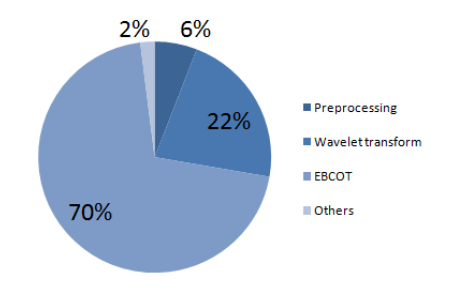
\includegraphics[width=\textwidth]{c1}
 		 \caption{Tiempos del proceso}
       	 \label{fig:c1}
  	 \end{subfigure}
   ~ 
	\begin{subfigure}[b]{0.48\textwidth}
		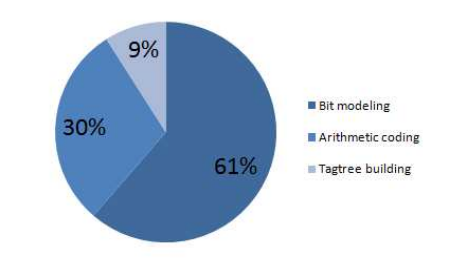
\includegraphics[width=\textwidth]{c2}
		\caption{Tiempos de EBCOT}
		\label{fig:c2}
	\end{subfigure}
	\caption{Distribución de tiempos de los procesos \cite{articulo}}
	\label{fig:circulos}
\end{figure}

Para la paralelización, se divide cada fotograma en recuadros, de manera que cada recuadro es asignado a un thread (cada uno con ID bidimensional). Se juntan 8 de dichos threads para formar un bloque y cada fotograma se divide en 30 bloques, todo para estar acordes con la arquitectura interna de la GPU. Debido a que la transformada ondícula es similar a una operación de convolución, se requiere información aledaña a cada recuadro por lo cual se dividen dichos recuadros de manera que exista un sobrelapamiento entre cada uno. Una vez terminado el procesamiento de cada recuadro (incluyendo los procesos interiores de EBCOT) se realiza la copia de información nuevamente al host para terminar el procesos de codificación. 

Una vez realizado el análisis, en \cite{articulo} se percataron de que mientras se realizaba el tagtree el GPU se quedaba en espera, mientras que cuando se realizaba el procesamiento en el GPU el CPU estaba en espera. Optimizando el tiempo de procesamiento, mientras el GPU está realizando los procesamientos, el CPU va realizando la división de recuadros del siguiente fotograma, mientras que cuando el CPU está realizando el tagtree, el GPU ya está realizando el procesamiento del siguiente fotograma.  Con este cambio, la utilización del dispositivo crece a un $82\%$.

Una vez analizados los tiempos después del paralelismo se obtuvo que el tiempo de codificación de 25 fotogramas fue de 4998ms; es decir 5.1 fotogramas por segundo, lo cual representa una mejoría de 20.7 veces el tiempo anterior.



%\nocite{*}
\bibliographystyle{apalike} %ORDENADOS!
\bibliography{references}
\end{document}	